\documentclass{standalone}
\usepackage{tikz}
\usepackage{amsmath}

\def\a{-50}
\def\d{4}
\def\w{15}
\def\h{75}
\def\b{500}
\def\scale{0.03}
\def\eps{0.5}

\def\aa{\a*\scale}
\def\dd{\d*\scale}
\def\ww{\w*\scale}
\def\hh{\h*\scale}
\def\bb{\b*\scale}

\begin{document}
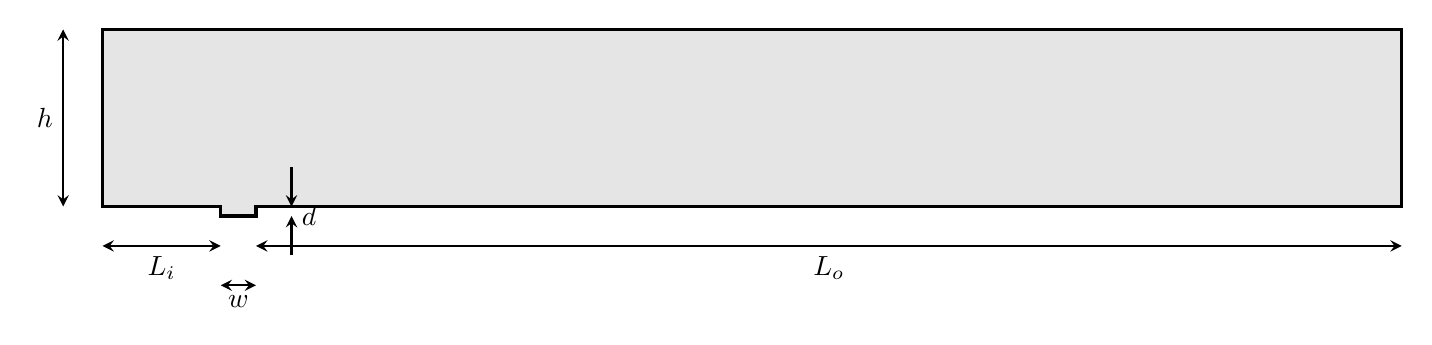
\begin{tikzpicture}[scale=1]
    % fill the rectangle
  \filldraw[fill=black!10, draw=black, line width = 1.25pt] (0,0) -- (0, -\dd) -- (\ww, -\dd) -- (\ww, 0) -- (\bb, 0) -- (\bb, \hh) -- (\aa, \hh) -- (\aa, 0) -- cycle;
    
    % arrows
  \draw[stealth-stealth, thick] (\aa-\eps, 0) -- (\aa-\eps, \hh) node[midway, left] {$h$};
  \draw[stealth-stealth, thick] (\aa, -\eps) -- (0, -\eps) node[midway, below] {$L_i$};
  \draw[stealth-stealth, thick] (\ww, -\eps) -- (\bb, -\eps) node[midway, below] {$L_o$};
  \draw[stealth-stealth, thick] (0, -2*\eps) -- (\ww, -2*\eps) node[midway, below] {$w$};

  %depth
  \def\xloc{2*\ww}
  \def\len{0.5}
  % node ate the end
  \draw[-stealth, thick] (\xloc, -\len-\dd) -- (\xloc, -\dd) node[above, anchor=west] {$d$};
  \draw[stealth-, thick] (\xloc, 0) -- (\xloc, \len);
\end{tikzpicture}
\end{document}
